
%%%%%%%%%%%%%%%%%%%%%%%%%%%%%%%%%%%%%%%%%%%%%%%%%%%%%%%%%%%%%%%%%%%%%%%%%%%%%%%%%%%%%
%
%  PLANTILLA DE TRABAJO DE GRADO
%  Universidad de San Buenaventura
%  By GHS & PADIA - 2026-2
%
%  Se recomienda compilar con XeLaTeX. Tambien funciona con pdfLaTeX
%  y con LuaLaTeX: la fuente se ajusta sola segun el motor.
%
%      latexmk main.tex          <- usa la configuracion de latexmkrc
%      make                      <- alternativa con make
%
%  En Overleaf: Menu > Settings > Compiler > XeLaTeX
%
%  Que se edita y donde:
%      parametros.tex            titulo, autores, asesor, programa, anio
%      sections/*.tex            un archivo por capitulo
%      anexos/anexos.tex         anexos A-E
%      bibs/sample.bib           referencias (estilo IEEE)
%      images/                   sus figuras
%      template/*.tex            formato: paquetes, fuentes, secciones, TOC, bibliografia
%
%%%%%%%%%%%%%%%%%%%%%%%%%%%%%%%%%%%%%%%%%%%%%%%%%%%%%%%%%%%%%%%%%%%%%%%%%%%%%%%%%%%%%

\documentclass[12pt]{article}
\usepackage[letterpaper, margin=2.5cm]{geometry}

% fuente principal del documento (Times New Roman o su equivalente libre)
%%%%%%%%%%%%%%%%%%%%%%%%%%%%%%%%%%%%%%%%%%%%%%%%%%%%%%%%%%%%%%%%%%%%%%%%%%%%%%%%%%%%%
%
%  PLANTILLA DE TRABAJO DE GRADO
%  Universidad de San Buenaventura
%  By GHS & PADIA - 2026-2
%
%%%%%%%%%%%%%%%%%%%%%%%%%%%%%%%%%%%%%%%%%%%%%%%%%%%%%%%%%%%%%%%%%%%%%%%%%%%%%%%%%%%%%
%%%%%%%%%%%%%%%%%%%%%%%%%%%%%%%%%%%%%%%%%%%%%%%%%%%%%%%%%%%%%%%%%%%%%%
%  Fuente del documento
%
%  Por defecto se usa TeX Gyre Termes: un clon libre de Times New Roman con
%  las mismas metricas (ocupa exactamente el mismo espacio en la pagina) que
%  viene incluido en todas las distribuciones de LaTeX y en Overleaf.
%
%  Se carga por nombre de archivo, no por nombre de fuente del sistema. Eso
%  es intencional: buscar fuentes del sistema obliga a XeLaTeX a recorrer el
%  catalogo de fuentes de la maquina, lo que en Overleaf puede tardar tanto
%  que la compilacion supera el limite de tiempo del plan gratuito.
%
%  Si trabaja en Windows o macOS y prefiere la Times New Roman autentica,
%  ponga el interruptor de abajo en \timesnewromantrue. En Overleaf dejelo
%  como esta.
%
%  La plantilla funciona con XeLaTeX, LuaLaTeX y pdfLaTeX: la fuente se
%  ajusta sola segun el motor.
%%%%%%%%%%%%%%%%%%%%%%%%%%%%%%%%%%%%%%%%%%%%%%%%%%%%%%%%%%%%%%%%%%%%%%

%  <<<<  interruptor: cambie a \timesnewromantrue para usar Times New Roman
\newif\iftimesnewroman
\timesnewromanfalse

\usepackage{iftex}

% verdadero con XeLaTeX o LuaLaTeX; falso con pdfLaTeX
\newif\ifmotormoderno
\ifXeTeX  \motormodernotrue \fi
\ifLuaTeX \motormodernotrue \fi

\ifmotormoderno
    %------------------------------------------------------------------
    %  XeLaTeX o LuaLaTeX
    %------------------------------------------------------------------
    \usepackage[no-math]{fontspec} % quite [no-math] si presenta errores

    \iftimesnewroman
        % fuentes instaladas en el sistema (Windows y macOS)
        \setmainfont{Times New Roman}
        \setmonofont{Courier New}[Scale=MatchLowercase]
    \else
        % clones libres, cargados por nombre de archivo (rapido, sin
        % consultar el catalogo de fuentes del sistema)
        \setmainfont{texgyretermes}[
            Extension      = .otf,
            UprightFont    = *-regular,
            BoldFont       = *-bold,
            ItalicFont     = *-italic,
            BoldItalicFont = *-bolditalic,
        ]
        \setmonofont{texgyrecursor}[
            Extension      = .otf,
            UprightFont    = *-regular,
            BoldFont       = *-bold,
            ItalicFont     = *-italic,
            BoldItalicFont = *-bolditalic,
            Scale          = MatchLowercase,
        ]
    \fi
\else
    %------------------------------------------------------------------
    %  pdfLaTeX: no puede usar fuentes del sistema, siempre usa los clones
    %------------------------------------------------------------------
    \usepackage[T1]{fontenc}
    \usepackage[utf8]{inputenc}
    \usepackage{tgtermes}          % clon libre de Times New Roman
    \usepackage{tgcursor}          % clon de Courier, para el codigo
    \renewcommand{\familydefault}{\rmdefault}
\fi


% paquetes de tablas, figuras, codigo, idioma, etc.
\input{template/packages.tex}

% referencias en estilo IEEE (biblatex + biber)
%%%%%%%%%%%%%%%%%%%%%%%%%%%%%%%%%%
% paquete para referencias
%%%%%%%%%%%%%%%%%%%%%%%%%%%%%%%%%%
\usepackage[style=ieee]{biblatex}
\addbibresource{bibs/sample.bib}   



% para que las urls tengan la misma fuente que resto del documento
%https://tex.stackexchange.com/questions/106622/how-to-change-the-font-of-url-in-the-bibliography
\usepackage{url}
\urlstyle{same}

%% coloca s.f cuando no tiene anio la referencia
%% https://copyprogramming.com/howto/biblatex-and-entries-with-no-date
%\newcommand{\mkbibnodate}{s\adddot f\adddot}
%\AtEveryCitekey{\iffieldundef{labelyear}{\restorefield{labelyear}{\mkbibnodate}}{}}
%\AtEveryBibitem{\iffieldundef{labelyear}{\restorefield{year}{\mkbibnodate}}{}}

% https://tex.stackexchange.com/questions/612417/biblatex-and-entries-with-no-date-part-2
\renewbibmacro*{date}{%
  \iffieldundef{year}
    {\bibstring{nodate}}
    {\printdate}}

\DeclareFieldFormat{url}{[Internet]\adddot\space\bibstring{urlfrom}\space\url{#1}}

\DeclareFieldFormat{urldate}{\adddot\addspace[\bibstring{urlseen}\addcolon\space #1]}

% puntos en cada entrada d la biliografia
\renewcommand*{\newunitpunct}{\addcomma\space}
%\renewcommand*{\newunitpunct}{\addperiod\space}
  
\DefineBibliographyStrings{spanish}{%
  urlfrom = {Disponible en},
  urlseen = {Consultado}
} 


\newbibmacro*{author+title+date}{%
  \ifnameundef{editor}
    {}
    {%
      \usebibmacro{editor}%
      \setunit{\addspace}%
      \printnames[byeditor]{editor}%
      \clearname{editor}%
      \newunit
    }%
  \usebibmacro{byeditorx}%
  \usebibmacro{bytranslator+others}%
  \ifnameundef{author}
  {%
    \printfield{title}
    \printtext[parens]{\usebibmacro{date}}
  }%
  {%
      \usebibmacro{author}\addcomma\space%
      \printtext[parens]{\usebibmacro{date}} \adddot \addspace %
      \printfield{title} \adddot
  }%
}



\DeclareBibliographyDriver{online}{%
  \usebibmacro{bibindex}%
  \usebibmacro{begentry}%
  %\usebibmacro{author/editor+others/translator+others}%
  \usebibmacro{author+title+date}%
  %\setunit{\adddot\addspace}% ELIMINADO
  %\usebibmacro{title}%        ELIMINADO  
  \setunit{\adddot\addspace}%
  \printlist{language}%
  \setunit{\adddot\addspace}%
  \usebibmacro{byauthor}%
  \setunit{\adddot\addspace}%
  \usebibmacro{byeditor+others}%
  \setunit{\adddot\addspace}%
  \printfield{version}%
  \setunit{\adddot\addspace}%
  \printfield{note}%
  \newunit\newblock
  \printlist{organization}%
  \setunit{\adddot\addspace}%
  \iftoggle{bbx:eprint}
    {\usebibmacro{eprint}}
    {}%
  \setunit{\adddot\addspace}%
  %\printtext[parens]{\usebibmacro{date}}% ELIMINDADO
  %\newunit\newblock                     % ELIMINDADO
  \usebibmacro{url+urldate}%
  \setunit{\adddot\addspace}%
  \usebibmacro{addendum+pubstate}%
  \setunit{\bibpagerefpunct}\newblock
  \usebibmacro{pageref}%
  \newunit\newblock
  \iftoggle{bbx:related}
    {\usebibmacro{related:init}%
     \usebibmacro{related}}
    {}%
  \usebibmacro{finentry}}


% formato de titulos y numeracion de capitulos y secciones
%%%%%%%%%%%%%%%%%%%%%%%%%%%%%
%  usa el paquete titlesec
%%%%%%%%%%%%%%%%%%%%%%%%%%%%

% Empezar sección en una nueva pagina
\let\stdsection\section
\renewcommand\section{\cleardoublepage\stdsection}

%----------------------------------
% NUMERACIÓN TIPO TESIS
%----------------------------------
\renewcommand{\thesection}{\arabic{section}}
\renewcommand{\thesubsection}{\thesection.\arabic{subsection}}
\renewcommand{\thesubsubsection}{\thesubsection.\arabic{subsubsection}}
\renewcommand{\theparagraph}{\thesubsubsection.\arabic{paragraph}}

%----------------------------------
% FORMATO DE SECCIONES
%----------------------------------
\titleformat{\section}[hang]
    {\filcenter\normalfont\normalsize\bfseries} % centrado
    {\thesection}
    {1em}{}

%----------------------------------
% FORMATO DE SUBSECCIONES
%----------------------------------
\titleformat{\subsection}[hang]
    {\normalfont\normalsize\bfseries}
    {\thesubsection}
    {1em}{}

%----------------------------------
% FORMATO DE SUBSUBSECCIONES
%----------------------------------
\titleformat{\subsubsection}[hang]
    {\normalfont\normalsize\bfseries}
    {\thesubsubsection}
    {1em}{}

\titlespacing{\subsubsection}{0cm}{*1}{*0.5}

%----------------------------------
% FORMATO DE PÁRRAFOS
%----------------------------------
\titleformat{\paragraph}[runin]
    {\normalfont\normalsize\itshape\bfseries}
    {\theparagraph}
    {1em}{}
    [:]

\titlespacing{\paragraph}{0cm}{*1}{*1}

% formato de la tabla de contenido, lista de figuras y lista de tablas
\input{template/toc.tex}

% comandos propios del template (\keywords, \palabrasclave, columnas P, etc.)
\input{template/config.tex}
\input{template/celdas.tex}

% datos del trabajo: titulo, autores, asesor, programa, anio
\newcommand{\autoresportada}{
Danna Andrea Rodriguez Galarcio\\
}

\newcommand{\autorescitacion}{
Nombre
}

\newcommand{\autorescitaciontexto}{
Nombre
}

\newcommand{\titulo}{Sistema de apoyo a la decisión basado en predicción de demanda para la gestión de inventarios}

\newcommand{\tituloencabezado}{Predicción de demanda para la gestión de inventarios}

\newcommand{\tipodocumento}{
Trabajo de grado presentado
%Trabajo de grado presentado
}

\newcommand{\tituloporoptar}{
ingeniero de sistemas
%ingeniero de sistemas
}

%%%%%%%%%%%%%%%%%%%%%%%%%%%%%%%%%%%%%%%
%           Asesor o asesores 
%%%%%%%%%%%%%%%%%%%%%%%%%%%%%%%%%%%%%%%

% si es un solo asesor cambielo a Asesor
\newcommand{\asesorpalabra}{Asesor}

\newcommand{\asesor}{
Ivan Mauricio Cabezas
}


\newcommand{\grado}{
Trabajo de grado profesional
}

\newcommand{\facultad}{
Facultad de Ingeniería (Cali)
}

\newcommand{\programa}{
Ingeniería Sistemas
}

\newcommand{\sede}{
Santiago de Cali, Colombia
}

\newcommand{\anio}{
2026
}





















%%%%%%%%%%%%%%%%%%%%%%%%%%%%%%%%%%%%%%%%%%%%%%%%%%%%%%%%%%%%%%%%%%%%%%
%  Interlineado 1.5 y espacio entre parrafos
%%%%%%%%%%%%%%%%%%%%%%%%%%%%%%%%%%%%%%%%%%%%%%%%%%%%%%%%%%%%%%%%%%%%%%
\usepackage{setspace}
\onehalfspacing
\setlength{\parskip}{1em}

%%%%%%%%%%%%%%%%%%%%%%%%%%%%%%%%%%%%%%%%%%%%%%%%%%%%%%%%%%%%%%%%%%%%%%
%  Justificacion sin division de palabras con guiones
%  https://sumanta679.wordpress.com/2009/05/20/latex-justify-without-hyphenation/
%%%%%%%%%%%%%%%%%%%%%%%%%%%%%%%%%%%%%%%%%%%%%%%%%%%%%%%%%%%%%%%%%%%%%%
\tolerance=1000
\emergencystretch=\maxdimen
\hyphenpenalty=10000
\hbadness=10000

%%%%%%%%%%%%%%%%%%%%%%%%%%%%%%%%%%%%%%%%%%%%%%%%%%%%%%%%%%%%%%%%%%%%%%
%  Enlaces internos (hyperref se carga de ultimo a proposito)
%%%%%%%%%%%%%%%%%%%%%%%%%%%%%%%%%%%%%%%%%%%%%%%%%%%%%%%%%%%%%%%%%%%%%%
\usepackage[linktoc=all]{hyperref}
\hypersetup{
    hidelinks,              % enlaces sin recuadro de color (para imprimir)
    pdftitle={\titulo},
    pdfauthor={\autorescitacion},
    bookmarksnumbered=true,
}

% descomente para ver los margenes y cajas de la pagina (util al ajustar el diseno)
%\usepackage{showframe}

%------------ Inicia Documento -------------------%
\begin{document} 

% las paginas preliminares (portada, legal, dedicatoria, indices) no llevan
% numero visible; la numeracion arabiga corre desde la primera pagina
\pagenumbering{arabic}
%%%%%%%%%%%%%%%%%%%%%%%%%%%%%%%%%%%%%%%%%%%%%%%%%%%%%%%%%%%%%%%%%%%%%%
%  Encabezado de pagina (paquetes fancyhdr y xcolor)
%    izquierda: titulo corto del trabajo   derecha: numero de pagina
%    debajo: una linea naranja
%%%%%%%%%%%%%%%%%%%%%%%%%%%%%%%%%%%%%%%%%%%%%%%%%%%%%%%%%%%%%%%%%%%%%%
\renewcommand{\headrulewidth}{1pt}
\renewcommand{\headrule}{\hbox to\headwidth{%
    \color{orange}\leaders\hrule height \headrulewidth\hfill}}

\fancyhead{}                                  % limpia el encabezado
\fancyhead[L]{\fontsize{10}{12}\selectfont \textcolor{gray}{\tituloencabezado}}
\fancyhead[R]{\textcolor{gray}{\thepage}}
\fancyfoot{}                                  % limpia el pie de pagina
\setlength{\headheight}{24.65pt}

\pagestyle{empty}   % en las paginas preliminares no se muestra el encabezado


%%%%%%%%%%%%%%%%%%%%%%%%%%%%%%%%%%%%%%%%%%%%%%%%%%%%%%%%%%%%%%%%%%%%%%
%  Portada, pagina legal y dedicatoria
%  (los datos se toman de parametros.tex)
%%%%%%%%%%%%%%%%%%%%%%%%%%%%%%%%%%%%%%%%%%%%%%%%%%%%%%%%%%%%%%%%%%%%%%
\input{templatepages/paginaportada}

\footnotesize                                  % la pagina legal va en 10 pt
\input{templatepages/paginalegal}
\normalsize

\input{templatepages/paginadedicatoria}


%%%%%%%%%%%%%%%%%%%%%%%%%%%%%%%%%%%%%%%%%%%%%%%%%%%%%%%%%%%%%%%%%%%%%%
%  Tabla de contenido, lista de tablas y lista de figuras
%%%%%%%%%%%%%%%%%%%%%%%%%%%%%%%%%%%%%%%%%%%%%%%%%%%%%%%%%%%%%%%%%%%%%%
\tableofcontents{}
\cleardoublepage{}

\listoftables
\cleardoublepage{}

\listoffigures



%%%%%%%%%%%%%%%%%%%%%%%%%%%%%%%%%%%%%%%%%%%%%%%%%%%%%%%%%%%%%%%%%%%%%%%%%%%%%%%%%%%%%
%  RESUMEN
%%%%%%%%%%%%%%%%%%%%%%%%%%%%%%%%%%%%%%%%%%%%%%%%%%%%%%%%%%%%%%%%%%%%%%%%%%%%%%%%%%%%%


\clearpage
\phantomsection                          % seccion sin numerar pero listada en el indice
\addcontentsline{toc}{section}{Resumen}
\section*{Resumen}

\pagestyle{fancy}   % a partir de aqui si se muestra el encabezado

resumen
\palabrasclave{Predicción de demanda, gestión de inventarios, sistemas de apoyo a la decisión, series de tiempo}

El presente proyecto tiene como objetivo desarrollar un sistema de apoyo a la decisión orientado a la predicción de la demanda de productos en los inventarios.

Esta problemática surge a partir de la falta de información precisa sobre las cantidades necesarias de productos, lo cual dificulta la correcta planificación y puede llevar a que halla desabastecimiento, afectando negativamente la atención de los clientes.

Para abordar esta situación, en este trabajo se propone el uso de modelos de predicción basados en datos históricos de consumo. El sistema permitirá estimar las cantidades requeridas de productos cada mes, así como generar indicadores que apoyen la toma de decisiones para los encargados del manejo del invertario, tales como puntos de reposición y alertas. 

Metodológicamente, se emplean diferentes tecnicas y enfoques de la ingenieria de sistemas para obtener esta  herramienta funcional, que contribuya a mejorar la gestión del inventario, optimizar la planificación de compras y reducir el riesgo de desabastecimiento.


%%%%%%%%%%%%%%%%%%%%%%%%%%%%%%%%%%%%%%%%%%%%%%%%%%%%%%%%%%%%%%%%%%%%%%%%%%%%%%%%%%%%%
%  ABSTRACT 
%%%%%%%%%%%%%%%%%%%%%%%%%%%%%%%%%%%%%%%%%%%%%%%%%%%%%%%%%%%%%%%%%%%%%%%%%%%%%%%%%%%%%

\clearpage
\phantomsection
\addcontentsline{toc}{section}{Abstract}
\section*{Abstract}

% el resumen en ingles se compone con las reglas tipograficas del ingles
\begin{otherlanguage}{english}
Abstract
\keywords{Demand forecasting, inventory management, decision support systems, time series}
The objective of this project is to develop a decision support system designed to predict demand for products in inventory.

This problem arises from a lack of accurate information regarding the required quantities of products, which hinders proper planning and can lead to shortages, negatively affecting customer service.

To address this situation, this study proposes the use of forecasting models based on historical consumption data. The system will enable the estimation of the required quantities of products each month, as well as the generation of indicators to support decision-making for inventory managers, such as reorder points and alerts.

Methodologically, various techniques and approaches from systems engineering are employed to develop this functional tool, which will help improve inventory management, optimize purchasing planning, and reduce the risk of stockouts.
\end{otherlanguage}


%%%%%%%%%%%%%%%%%%%%%%%%%%%%%%%%%%%%%%%%%%%%%%%%%%%%%%%%%%%%%%%%%%%%%%%%%%%%%%%%%%%%%
%  GLOSARIO
%%%%%%%%%%%%%%%%%%%%%%%%%%%%%%%%%%%%%%%%%%%%%%%%%%%%%%%%%%%%%%%%%%%%%%%%%%%%%%%%%%%%%

\clearpage
\phantomsection
\addcontentsline{toc}{section}{Glosario}
\section*{Glosario}

Demanda:
Cantidad de productos requeridos durante un período determinado, calculada a partir del comportamiento histórico de consumo o ventas.

Predicción de demanda:
Proceso mediante el cual se estiman las cantidades futuras de productos utilizando modelos estadísticos o de aprendizaje automático basados en datos históricos.

Gestión de inventarios:
Conjunto de actividades orientadas al control, almacenamiento, abastecimiento y seguimiento de los productos disponibles en una organización.

Inventario
Conjunto de productos, materiales o recursos almacenados y disponibles para su uso, venta o distribución.

Desabastecimiento:
Situación en la que un producto no se encuentra disponible en el inventario cuando es requerido.

Sistema de apoyo a la decisión:
Herramienta informática diseñada para asistir a los usuarios en la toma de decisiones mediante el análisis de datos y la generación de información relevante.

Modelo de predicción:
Algoritmo o método matemático utilizado para estimar valores futuros a partir de datos históricos y patrones identificados en la información.

Datos históricos:
Registros de consumo, ventas, compras o movimientos de inventario ocurridos en períodos anteriores y utilizados para el análisis y la predicción.

Punto de reposición:
Nivel de inventario a partir del cual se debe realizar un nuevo pedido para evitar el desabastecimiento.

Tiempo de entrega (Lead Time):
Período que transcurre entre la realización de un pedido y la recepción efectiva de los productos solicitados.

Series de tiempo:
Conjunto de observaciones registradas en orden cronológico que permiten analizar patrones, tendencias y comportamientos a lo largo del tiempo.

Aprendizaje automático (Machine Learning):
Rama de la inteligencia artificial que permite a los sistemas aprender patrones a partir de datos y realizar predicciones sin ser programados explícitamente para cada situación.

Dominio de inventario:
Contexto o sector específico en el que se gestionan inventarios, como retail, manufactura, logística, salud, restaurantes o comercio electrónico.


%%%%%%%%%%%%%%%%%%%%%%%%%%%%%%%%%%%%%%%%%%%%%%%%%%%%%%%%%%%%%%%%%%%%%%%%%%%%%%%%%%%%%
%  CAPITULOS
%  cada archivo contiene el titulo del capitulo (\section) y todas sus
%  subsecciones. Para reordenar o quitar un capitulo, mueva o comente su \input.
%%%%%%%%%%%%%%%%%%%%%%%%%%%%%%%%%%%%%%%%%%%%%%%%%%%%%%%%%%%%%%%%%%%%%%%%%%%%%%%%%%%%%

\section{Capítulo 1: Introducción}

\subsection{Contexto}
La gestion eficiente de inventarios supone un desafio constante en diversos sectores. Problemas como sufrir de debastabecimiento pueden surgir por distintos factores como retradsos en la entrega por parte de los proovedores, variaciones inesperadas de la demanda, o deficiencias en los procesos de planificacion. Estas situaciones, en muchos casos, se encuentran fuera del control de los administradores, lo que incrementa la complejidad para ellos a la hora de tomar desiciones relacionadas con el abastecimiento.

Actualmente, normalmente en muchas empresas se cuenta con un software para gestion de inventarios tipo ERP, con este software se administra la disponibilidad de los productos mediante el uso de diferentes tipos de movimientos de inventario:

Uno de los tipos de movimientos consiste en las entradas de inventario, las cuales responden a la adquisicion de productos atraves de proovedores y son registradas mediante facturas que incluyen informacion como fecha, proovedor y costo. 

Por otro lado, estan las salidas por consumo, las cuales representan la venta, distribución o consumo de los productos, registrando información relacionada con las cantidades entregadas y el destino de estas. Adicionalmente, existen salidas de inventario asociadas a sucesos como devoluciones, productos dañados, vencimientos, pérdidas o ajustes de inventario, se regista la cantidad de productos que deben de ser retirados del inventario junto con su respectivo motivo. Posteriormente, se realizan ajustes de inventario, los cuales pueden ser tanto positivos como negativos, con el fin de corregir diferencias entre las cantidades resgistradas den el sistema y las existencias reales, garantizando asi la consistencia de la informacion.

En general, un buen analisis de estos movimientos resulta fundamental para comprender el comportamiento del consumo de productos y asi mejorar los procesos de planificacion del abastecimiento.

\subsection{Planteamiento del Problema}
En diferentes entornos, existe una problemática en la que la gestión del inventario de productos se ve afectado debido a la falta de información precisa sobre la demanda mensual de los mismos, lo que dificulta la planificación adecuada del abastecimiento. En este contexto, surge la necesidad de contar con herramientas que permitan analizar los datos históricos de inventario y generar estimaciones de demanda que apoyen la toma de decisiones relacionadas con el abastecimiento.

\begin{figure}[H]
    \centering
    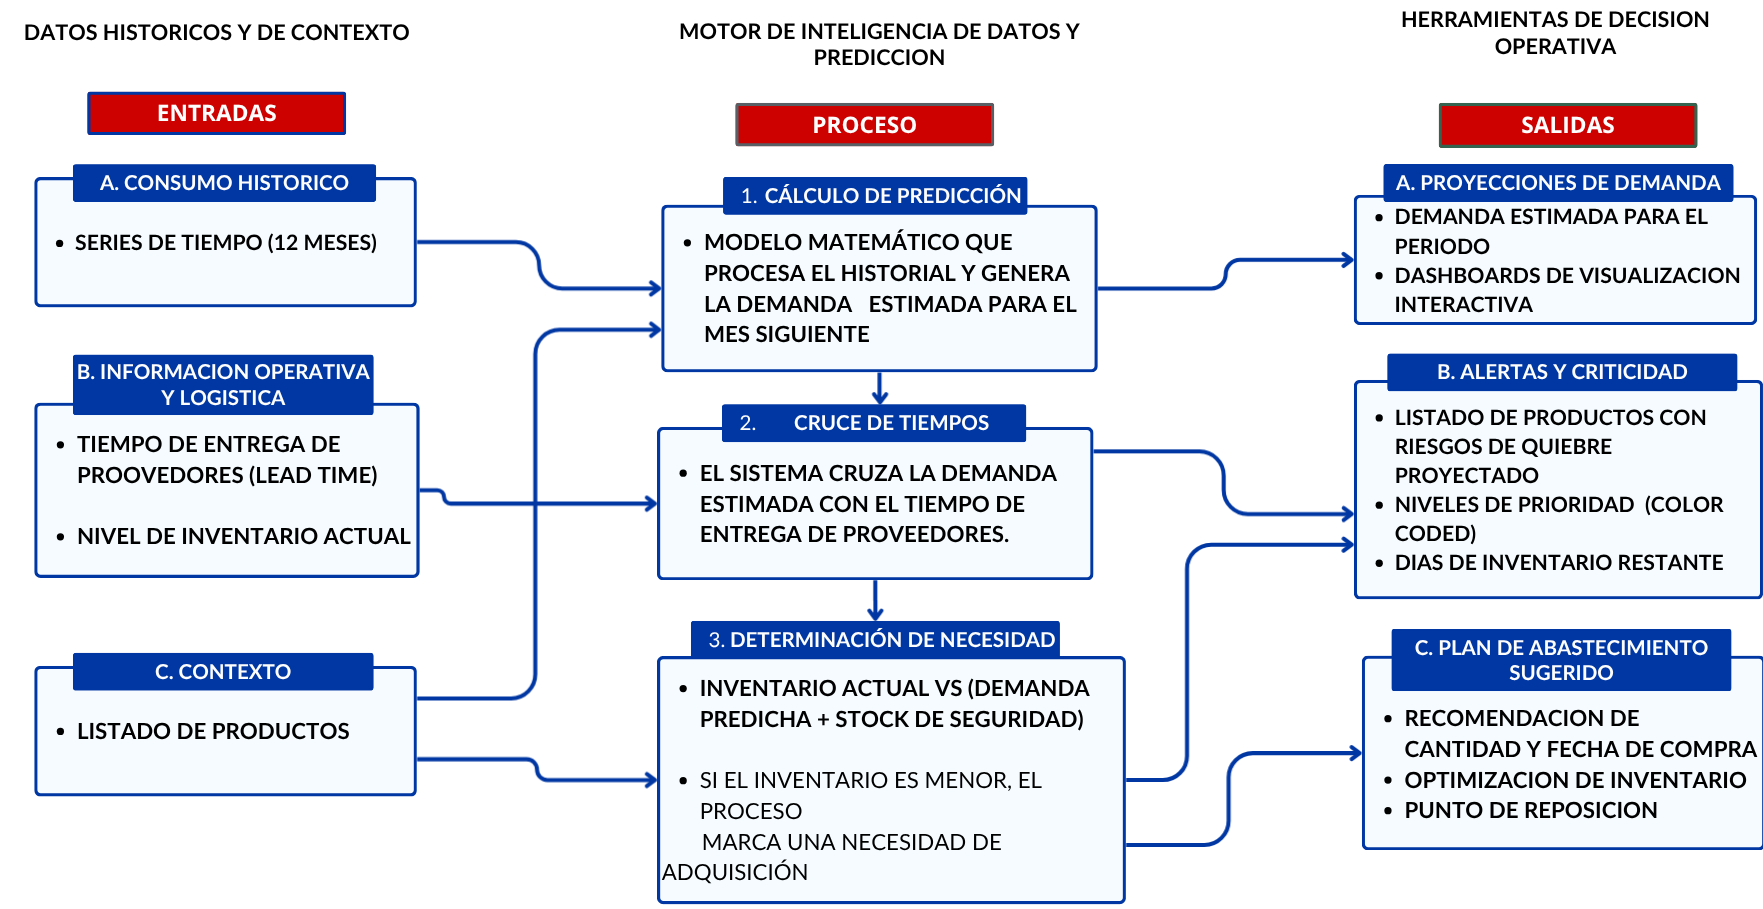
\includegraphics[width=1.0\textwidth]{templatefigures/entradas_salidas.png}
    \caption{Esquema detallado de entradas, proceso y salidas del sistema.}
\end{figure}

\subsection{Justificación del Problema}
Este proyecto se justifica teniendo en cuenta que esta es una problemática que no se ha visto abordada a profundidad y continua siendo una dificultad para organizaciones de diferentes sectores. Además este proyecto permite aplicar conocimientos de la ingenieria de sistemas como analisis de datos, modelos de prediccion y aprendizaje automatico para la construccion de una herramienta que contribuya a mejorar los procesos de planificacion y administracion, generando beneficios tanto para las organizaciones y los usuarios finales.

\subsubsection{IMPACTOS}

Mejorar la disponibilidad de los productos mediante una mejor planificación de los inventarios, apoyar la toma de decisiones del personal encargado del abastecimiento,y fortalecer el uso de herramientas tecnológicas en el sector administrativo.


\subsection{Propuesta de Solución}
Con este proyecto se propone el desarrollo de un software que ayude a predecir la demanda de productos en diferentes dominios y contetos de gestion de inventarios. Este sistema se realizara tras analizar datos como historial de consumo, esto para poder estimar exactamente las cantidades necesarias de cada producto en periodos mensuales.

La solucion implementara modelos de prediccion de demanda que procesaran la informacion historica para identificar patrones y en base a ellos, generar estimaciones futuras. A partir de estas predicciones, el sistema podra proporcionar informacion relevante para la toma de decisiones, tales como cantidades recomendadas de compra, puntos de reposicion y posibles alertas de desabastecimiento.

Se utilizaran datos reales del año 2021 del sector salud como caso de estudio, que seran complementados con datasets con datos publicos de diferentes dominios esto para poder evaluar el comportamiento del sistema en diferentes contextos.

Adicionalmente, el sistema tendra en cuenta variables como tiempo de entrega de proovedores (lead time) y cantidad de productos disponivle, con el proposito de lograr que el sistema sea lo mas preciso posible.

Esta informacion sera presentada en una interaz que permitira visualizar los resultados de manera comprensible, esto para facilitar su uso por parte del personal encargado de la gestion de inventarios.
\begin{figure}[H]
    \centering
    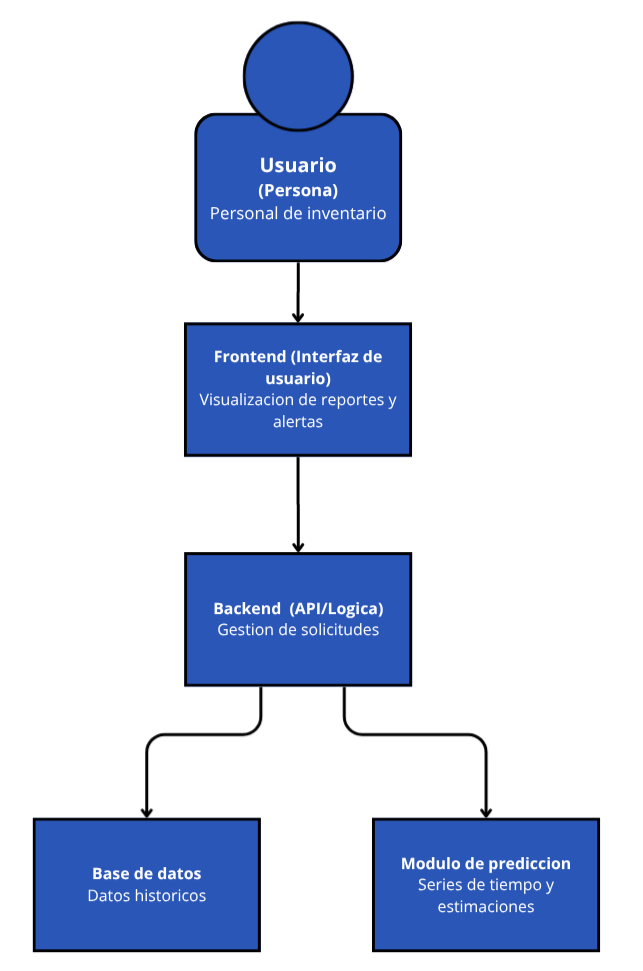
\includegraphics[width=0.5\textwidth]{templatefigures/propuesta.png}
    \caption{Esquema detallado de la propuesta de solucion.}
\end{figure}

\subsection{Pregunta de Investigación}
¿Cómo se puede diseñar e implementar un sistema de apoyo a la decisión que, mediante modelos de predicción de demanda, permita estimar las cantidades necesarias de productos en un sistema de gestion de inventarios?

% \subsubsection{ESTRUCTURACION DE LA PREGUNTA MEDIANTE PICO}

% Con el fin de estructurar de manera formal la pregunta de investigación, se empleo la metodología PICO (Population, Intervention, Context, Outcome). Esta metodología ayuda a  identificar los elementos clave del problema y orientar el desarrollo de la solución propuesta.

% \begin{itemize}
%     \item \textbf{P (Population):} Sistemas de gestión de inventario de diferentes dominios.
    
%     \item \textbf{I (Intervention):} Implementación de un sistema de apoyo a la decisión basado en modelos de predicción de demanda.
    
%     \item \textbf{C (Context):} Proceso de planificación y adquisición de productos dentro de un sistema de gestion de inventarios.
    
%     \item \textbf{O (Outcome):} Generación de estimaciones de demanda que apoyen la toma de decisiones en la gestión de inventarios.
% \end{itemize}

\subsubsection{Preguntas Derivadas}

¿Qué variables y datos históricos son necesarios para estimar la demanda mensual de productos?

¿Qué modelos de predicción de demanda son más adecuados para estimar el consumo o venta de productos en diferentes dominios?

¿Cómo debe estructurarse el proceso de análisis y procesamiento de datos para generar predicciones confiables?

¿Qué tipo de salidas debe generar el sistema (por ejemplo, cantidades estimadas, punto de reposición, alertas) para apoyar la toma de decisiones?


\subsection{Objetivos}
\input{sections/objetivos.tex}
\subsubsection{OBJETIVO GENERAL}
Desarrollar un sistema que le permita a los usuarios poder predecir cual va a ser la demanda mensual de productos mediante el analisis de datos historicos, para garantizar su correcta planificacion y abastecimiento

\subsubsection{Objetivos Específicos}

Identificar las fuentes de datos relevantes, incluyendo el historial de consumo y las variables del inventario necesarias para la predicción de la demanda de productos.

Seleccionar modelos de predicción de demanda adecuados para estimar el consumo o venta mensual de productos en diferentes contextos de los inventarios.

Incorporar variables como el tiempo de entrega de proveedores y el punto de reposición dentro del sistema para complementar las estimaciones de demanda.

Diseñar un módulo de visualización que presente las predicciones de manera clara y comprensible para apoyar la toma de decisiones del usuario.

Evaluar el desempeño del sistema desarrollado mediante la realización de pruebas con datos históricos, con el fin de analizar la precisión de las predicciones generadas y verificar su utilidad en el apoyo a la toma de decisiones en la gestión del inventario.

\subsection{Restricciones}
El proyecto tiene como principal alcance el desarrollo de un sistema de apoyo a la decisión orientado a la predicción de la demanda de medicamentos críticos en una farmacia hospitalaria, esto utilizando los datos históricos de consumo como principal fuente de información. El sistema permitirá estimar la cantidad mensual requerida de medicamentos mediante la implementación de modelos de predicción de demanda, integrando funcionalidades como visualización de resultados, generación de reportes y apoyo en la toma de decisiones relacionadas con la planificación del abastecimiento. Asimismo, el sistema proporcionara al usuario cálculos como el punto de reposición, con el fin de contribuir a una mejor organización y control de los recursos disponibles en los entornos hospitalario.

El desarrollo del proyecto presenta algunas restricciones que deben ser consideradas. En primer lugar, el sistema se basará en un conjunto de datos históricos reales de la Clínica Nuestra señora de los remedios limitado al año 2021, lo que puede afectar la capacidad del modelo para capturar comportamientos actuales o cambios en la demanda a lo largo del tiempo. Además, no se contará con integración en tiempo real con sistemas hospitalarios, por lo que las predicciones se realizarán sobre datos estáticos.

\subsection{Recursos y Viabilidad Técnica}
\input{sections/recursos_viabilidad.tex}

\section{Capítulo 2: Marco de Referencia}

Para la construcción del estado del arte, se realizó una revisión de literatura en bases de datos académicas reconocidas, con el fin de identificar estudios relevantes relacionados con la predicción de demanda y la gestión de inventarios en el sector salud.

\subsubsection{Criterios de inclusión}

Se consideraron los siguientes criterios para la selección de los estudios:

\begin{itemize}
    \item Trabajos disponibles en español o inglés.
    \item Publicaciones académicas en bases de datos como IEEE Xplore, Scopus, ScienceDirect, Google Scholar y repositorios institucionales.
    \item Estudios enfocados en gestión de inventarios.
    \item Investigaciones que utilicen modelos de predicción de demanda.
    \item Estudios que describan el diseño de sistemas informáticos de apoyo a la decisión.
\end{itemize}

\subsubsection{Criterios de exclusión}

Se excluyeron los estudios que cumplían con las siguientes características:

\begin{itemize}
    \item Estudios con más de 10 años de antigüedad.
    \item Documentos incompletos o resúmenes sin acceso al texto completo.
\end{itemize}

\subsection{Fundamentos Teóricos}
\subsubsection{Gestion de inventarios}

La gestion de inventarios consiste en el proceso que se realiza sobre la mercancia para conocer la cantidad disponible, esto permitiendo analizar los niveles de existencia y la aproximacion del consumo real.\cite{meana2024gestión}

Los pasos basicos para realizar una correcta gestion de inventario consiste en: Compra del inventario, en el que los productos se entregan al almacen o punto de venta, Almacenamiento del inventario, en el que este se guarda hasta que se necesite y Aprovechamiento del inventario, en donde se controla la cantidad de productos que hay a la venta para finalmente enviarlo o venderlo a los clientes.\cite{ibm_inventario}

\paragraph{Tipos de gestion de inventario}

\begin{description}
    \item[Gestión periódica de inventarios] Este método implica realizar un recuento físico del inventario a intervalos específicos. Se toma el inventario al inicio del periodo, se suman las nuevas compras y se deduce el inventario final para calcular el costo de las mercancías vendidas (COGS).\cite{ibm_inventario}

    \item[Gestión de inventario de códigos de barras] Utiliza un sistema que asigna un número único a cada producto. Permite asociar datos como proveedor, dimensiones del producto, peso y cantidad en stock.\cite{ibm_inventario}

    \item[Gestión de inventario RFID] Transmite de forma inalámbrica la identidad de un producto mediante un número de serie único. Mejora la eficiencia y visibilidad del inventario, facilitando el seguimiento de artículos.\cite{ibm_inventario}
    
\end{description}

\subsubsection{Prediccion de demanda}

La prediccion de la demanda es un proceso que permite mejorar la gestion de los niveles de inventario mediante la utilizacion de datos historicos. Una correcta prediccion de la demanda le permite a las organizaciones el poder tomar decisiones mas inteligentes a la hora de manejar sus provisiones, evitando la falta o exceso de productos, de esta manera, aumentando tanto la satisfaccion del cliente como la creacion de estraregias de negocio mas efectivas a corto y largo plazo \cite{ibm_prevision_demanda}.

En los ultimos años, los mercados han evolucionado y se han vuelto cada vez mas exigentes en cuanto la calidad y precicion de los servicios, es por eso, que muchas organizaciones se ha visto inclinadas a incluir el uso de nuevas herramientas y tecnologias como Inteligencia Artificial. Machine Learning o analisis predictivo, para automatizar y perfeccionar esta tarea, ya que los metodos actuales estaticos que son la norma en muchas empresas y organizaciones han empezado a quedar obsoletas para satisfacer las necesidades del mercado actual.\cite{ibm_prevision_demanda, valencia2015}

La principal debilidad de los modelos de inventario actuales es que al ser poco robustos, no toman en contemplacion diferentes factores externos de manera inteligente \cite{valencia2015}. 

\subsubsection{Series de tiempo}

Las series temporales son usadas para analizar datos históricos recogidos en intervalos regulares, como ventas diarias o mensuales, para identificar patrones, tendencias estacionales y ciclos. Estos patrones se identifican mediante técnicas como gráficos ACF y PACF, tambien estos patrones sirven para ajustar modelos estadísticos o de aprendizaje automático (como ARIMA, SARIMAX o Prophet) que permiten proyectar valores futuros \cite{10596_69801}

Se utilizan estos modelos para hacer predicciones, los datos se agrupan en intervalos (mensualmente) para reducir variabilidad y facilitar el análisis. Tras el análisis de datos, se ajustan los modelos y se evalúan mediante métricas como el RMSE, para que las predicciones sirvan en la toma de decisiones de gestión y planificación de recursos


\subsubsection{Modelos de prediccion de demanda}

\paragraph{Redes Neuronales Artificiales (RNA)}\mbox{}\\
Las redes neuronales artificiales (RNA) son técnicas útiles para la previsión de la demanda, gracias a su capacidad para manejar datos no lineales y captar relaciones funcionales sutiles entre datos empíricos, incluso cuando las relaciones subyacentes son desconocidas o difíciles de describir.

    \subparagraph{Long Short-Term Memory (LSTM)}\mbox{}\\
    Las redes neuronales de memoria a largo y corto plazo o LSTM es un tipo de red neuronal que se ha demostrado eficaz en la predicción de series temporales, esta tecnica esta diseñada para procesar datos secuenciales y temporales que fue creada para superar las limitaciones de las redes neuronales tradicionales.\cite{10124729}.

    Su funcionamiento se basa en una estrictura de memoria que permite a la red aprender y recordar información a lo largo del tiempo, lo que es especialmente útil para capturar dependencias a largo plazo en los datos. LSTM cuenta con las tres siguientes puertas: 

    \begin{description}
        \item[Puerta de olvido (forget gate):] Decide qué información se descarta. Esta se calcula mediante la función sigmoide, que toma como entrada el vector de entrada actual y el estado oculto anterior, de esta menra, generando un valor entre 0 y 1 para cada componente de la celda de la memoria. 
        
        \begin{equation}
        f_t = \delta(W_f[h_{t-1}, X_t] + b_f)
        \end{equation}   

        \item[Puerta de entrada (input gate):] Decide qué información se almacena en la memoria. Tambien usa una funcion tanh para normalizar la informacion que pasa atraves de la red neuronal.
        \begin{equation}
        i_t = \delta(W_i[h_{t-1}, X_t] + b_i), \quad L_t = \tanh(W_c[h_{t-1}, X_t] + b_c)
        \end{equation}

        \item[Puerta de salida (output gate):] Decide qué información se utiliza para generar la salida oculta actual.
        \begin{equation}
        o_t = \delta(W_o[h_{t-1}, X_t] + b_o)
        \end{equation}

        La actualizacion del estado celular se realiza mediante:

        \begin{equation}
        C_t = f_t * C_{t-1} + i_t * L_t
        \end{equation}

        Finalmente, la salida oculta se calcula aplicando la funcion tanh al estado celular y multiplicandolo por la puerta de salida como:
        \begin{equation}
        h_t = o_t * \tanh(C_t)
        \end{equation}
    \end{description}


    \subparagraph{Gated Recurrent Unit (GRU)}\mbox{}\\
    Gru es modelo de prediccion bastante parecido a LSTM, pero con una arquitectura mucho mas simple, lo que la hace muchisimo mas compacta y potencialmente menos costosa computacionalmente que una LSTM equivalente. Estas han demostrado tener exito en diferentes aplicaciones relacionadas con datos secuenciales o temporales, principalmente si son secuencias largas. GRU reduce el numero de tres redes compuestas distintas que usa LSTM en solo 2, esto mediante la combinacion de la compuerta de entrada y la compuerta de olvido mediante una suma directa. Las compuertas de GRU se denominan: Compuerta de actualizacion y Compuerta de reinicio. \cite{Salem2022}

    El modelo GRU se presenta como:

    \begin{equation}
        h_t = g(Uh(r_t \odot h_{t-1}) + Wx_t + b_h)
    \end{equation}

    \begin{equation}
    h_t = (1 - z_t) \odot h_{t-1} + z_t \odot \tilde{h}_t
    \end{equation}
    donde $z_t$ es la compuerta de actualización, $r_t$ es la compuerta de reinicio y $\tilde{h}_t$ es la propuesta de nueva información. Las dos compuertas se presentan como:

    \begin{equation}
        z_t = \sigma (U_z h_{t-1} + W_z x_t + b_z)
    \end{equation}

    \begin{equation}
        r_t = \sigma (U_r h_{t-1} + W_r x_t + b_r)
    \end{equation}

\paragraph{Modelos estadísticos y de Machine Learning tradicionales}
    \subparagraph{Regresión lineal}\mbox{}\\
    Los modelos de regresion son utilizados para resolver problemas de prediccion, el objetivo de este modelo puede ser explicativo, donde se busca, por ejempo, evaluar como ciertas variables independientes afectan a una variable dependiente, o predictivo, en el que se busca estimar el valor de la variable dependiente en funcion de las independientes \cite{pelaez2016modelos}.

    Un modelo de regresion se expresa como: 

    \begin{equation}
    y = (x_1, x_2, ..., x_n) \beta + \epsilon
    \end{equation}

    Existen distintas opciones para poder estimar un modelo de regresion, siendo las mas comunes: Regresion lineal  y regresion logistica. La eleccion depende del tipo de variable dependiente que se tenga, si es una variable continua se utiliza regresion lineal, mientras que si se trata de una variable dicotomica se utiliza una variable dicotomica.

\paragraph{Modelos basados en árboles de decisión}
    \subparagraph{XGBoost}\mbox{}\\
    XGBoost se ha utilizado ampliamente en numerosos campos para lograr resultados de vanguardia (state-of-the-art) en tareas relacionadas con datos y predicción. Su funcionamiento consiste en en un sistema de aprendizaje automatizado basado en el metodo de Tree Boosting que incluye un algoritmo de aprendizaje de arboles. EL Tree Boosting es un algoritmo de aprendizaje por conjuntos o ensemble learning, capaz de transformar varios clasificadores debiles en uno fuerte con el objetivo de obtener un mejor rendimiento en le clasificacion, es decir, se combinan multiples arboles para obtener un modelo mas potente. Un modelo tree boosting se escribe de la siguiente manera\cite{ren2017novel}:

    \begin{equation}
        \hat{y_i} = \sum_{k=1}^{K} f_k(x_i), f_k \in F
    \end{equation}
    
    Donde:
    \begin{equation}
        F = \{f(x) = w_{q(x)}\} (q: R^m \rightarrow T, w \in R^T)
    \end{equation}
    
    Representa el espacio de los arboles de regresion o clasifiacion

\subsection{Antecedentes}
\subsubsection{Comparación de modelos de predicción de demanda}

Debido a que existen diferentes modelos y tecnicas para la prediccion de la demanda, se realizo una revision de literatura de diferentes estudios que emplean los modelos mas utilizados para la prediccion de la demanda, esto con el fin de realizar el siguiente analisis comparativo para determinar cual es el mas adecuado para la prediccion de demanda en el presente proyecto, teniendo en cuenta ventajas, limitaciones y caracteristicas como: tipo de datos utilizados, dominio de aplicación, tecnica de aplicacion, metricas de evaluacion y resultados obtenidos, dataset utilizado, entre otros.

\begin{table}[H]
\centering
\caption{Comparación de técnicas de predicción aplicadas a problemas de demanda y series de tiempo}
\label{tab:comparacion_modelos}
\renewcommand{\arraystretch}{1.3}
\small

\resizebox{\textwidth}{!}{%
\begin{tabular}{|p{2.5cm}|p{4.5cm}|p{4.5cm}|p{4.5cm}|p{4.5cm}|p{4.5cm}|}
\hline

\textbf{Aspecto} &
\textbf{Redes neuronales (ANN)} &
\textbf{LSTM} &
\textbf{Regresión lineal} &
\textbf{GRU} &
\textbf{XGBoost} \\ 
\hline

\textbf{Referencia} &
\textit{Demand Forecasting Using Neural Network for Supply Chain Management} &
\textit{LSTM Model Based Demand Forecasting in Supply Chain Using Efficient Optimizer} &
\textit{Application of ABC Analysis and Linear Regression Model in Inventory Management} &
\textit{StockNet--GRU Based Stock Index Prediction} &
\textit{XGBoost-Based Demand Forecasting in Supply Chain Management Using Machine Learning Algorithm} \\ 
\hline

\textbf{Datos utilizados} &
Datos históricos de ventas organizados como series de tiempo. Se emplean ventas mensuales de un filtro de combustible entre 2011 y 2013 para predecir la demanda de 2014. &
Datos históricos de ventas organizados como series de tiempo. Incluyen fecha, unidades vendidas, ganancias y ubicación, seleccionando las variables relevantes para el entrenamiento. &
Datos históricos de inventario y ventas. Incluyen información de productos, inventario, órdenes de compra y venta, cantidad y precio de venta, fecha, marcas, clasificación e impuestos. &
Series de tiempo financieras correspondientes a precios históricos de apertura del índice bursátil CNX Nifty y de las 10 acciones con mayor correlación. Los datos se normalizan y organizan mediante ventanas deslizantes de 20 días. &
Datos logísticos y de cadena de suministro relacionados con la demanda, incluyendo variables asociadas con proveedores y logística. Los datos se normalizan mediante Z-score y posteriormente se seleccionan las variables relevantes. \\ 
\hline

\textbf{Dominio} &
Gestión de la cadena de suministro, control de inventarios, manufactura y distribución. También presenta aplicaciones en turismo, consumo eléctrico, supermercados y ventas. &
Gestión de la cadena de suministro y predicción de demanda. &
Gestión de inventarios, cadena de suministro y análisis de ventas. &
Predicción de índices bursátiles, mercados financieros y análisis de series de tiempo. &
Gestión de la cadena de suministro, predicción de demanda, logística y optimización de inventarios. El enfoque puede aplicarse a diferentes sectores que requieran pronósticos de demanda. \\ 
\hline

\textbf{Técnica} &
Red neuronal \textit{feed-forward} entrenada mediante \textit{Backpropagation}. Se comparan Gradient Descent, Conjugate Gradient y Levenberg--Marquardt, siendo este último el de mejor desempeño. &
Red neuronal recurrente LSTM con tres capas, regularización mediante Dropout y optimizadores Adam y SGD. Se experimenta con épocas, tasa de aprendizaje, tamaño de lote y longitud de secuencia. &
Modelo de regresión lineal para identificar tendencias en cantidad y precio de venta. Utiliza Gradient Descent para minimizar el error cuadrático, después de realizar limpieza de datos y selección de variables. &
Red neuronal recurrente GRU integrada en la arquitectura StockNet. Utiliza ventanas deslizantes de 20 días, optimizador Adam, activación ReLU y datos normalizados entre 0 y 1. &
El proceso incluye normalización Z-score, selección de características mediante un Algoritmo Genético, predicción mediante XGBoost y optimización de hiperparámetros mediante Particle Swarm Optimization (PSO). \\ 
\hline

\textbf{Métricas} &
Error absoluto de pronóstico (\textit{Forecasting Error}) y porcentaje de error, comparando los valores pronosticados con los valores reales. &
RMSE para medir la diferencia entre valores reales y predichos. También se compara el tiempo promedio por época para evaluar la eficiencia computacional. &
Coeficiente de determinación ($R^2$). El estudio reporta un valor de 70,57\,\% para la predicción de la cantidad vendida y cercano al 80\,\% para el precio de venta. &
RMSE, MAE y MAPE. También se considera el tiempo de ejecución y se utiliza la prueba estadística de Wilcoxon para validar diferencias entre modelos. &
MAE, RMSE y coeficiente de determinación. Se compara el desempeño de XGBoost con SARIMA, Decision Tree (DT) y Random Forest (RF). \\ 
\hline

\textbf{Dataset} &
Datos reales de consumo mensual de un filtro de combustible perteneciente a una empresa manufacturera. Contiene registros mensuales entre 2011 y 2013 para entrenamiento y validación. &
\textit{Sales Dataset} con información histórica de ventas utilizada para entrenar y evaluar el modelo. &
Dataset de inventario de una tienda de comestibles (\textit{grocery store}) con información de productos, inventario y ventas. Después del preprocesamiento se utilizan aproximadamente 60 observaciones correspondientes a dos meses. &
Índice bursátil CNX Nifty y las 10 acciones más correlacionadas del National Stock Exchange (NSE) de India, obtenidos desde Yahoo Finance. Contiene 5.904 días de negociación entre abril de 1996 y enero de 2020. &
Dataset de demanda de cadena de suministro con información relacionada con logística y proveedores. Se utiliza para entrenar y evaluar el modelo de predicción. \\ 
\hline

\textbf{Comentario / reseña} &
Las ANN permiten modelar relaciones no lineales y presentan resultados favorables frente a métodos tradicionales de series de tiempo. Son útiles para predicciones de corto plazo, aunque requieren suficiente información y ajuste de parámetros. &
LSTM constituye una alternativa eficaz para la predicción de demanda debido a su capacidad para capturar dependencias temporales de largo plazo. Puede contribuir a la optimización de inventarios y a la toma de decisiones en la cadena de suministro. &
La regresión lineal permite identificar y proyectar tendencias generales de ventas e inventario y presenta una menor complejidad. Sin embargo, tiene limitaciones para representar relaciones complejas y eventos extraordinarios. &
GRU permite capturar dependencias temporales y presenta resultados favorables en la predicción de series de tiempo. Sin embargo, el estudio analizado se desarrolla en el dominio financiero, por lo que su aplicación a inventarios requiere evaluación adicional. &
XGBoost presenta capacidad para modelar relaciones complejas y puede utilizarse para apoyar la planificación de inventarios, reducir costos y optimizar operaciones en la cadena de suministro. \\ 
\hline

\end{tabular}%
}

\vspace{0.2cm}

\begin{flushleft}
\footnotesize
\textit{Fuente: Elaboración propia a partir de los estudios revisados.}
\end{flushleft}

\end{table}

\subsubsection{Implementaciones de referencia consultadas}

Ademas de los estudios academicos revisados en la Seccion 2.2.1, se consultaron cuatro implementaciones practicas de codigo abierto, disponibles en Kaggle y GitHub, que sirvieron como base y punto de partida para la construccion del pipeline de prediccion de Thary. La Tabla \ref{tab:implementaciones_referencia} resume cada una de estas implementaciones, el identificador que se usara para referirse a ellas a lo largo del documento, y el aporte que realizaron al diseño del sistema.

\begin{table}[H]
    \centering
    \caption{Implementaciones de referencia consultadas para el desarrollo de Thary.}
    \label{tab:implementaciones_referencia}
    \begin{tabularx}{\textwidth}{lp{2.2cm}XX}
        \toprule
        \textbf{ID} & \textbf{Autor} & \textbf{Título} & \textbf{Aporte a Thary} \\
        \midrule
        Ejemplo 1 (SKU Demand Forecasting) & Dhruvi Shah \cite{ejemplo1_demandforecast} & \textit{Demand Forecasting \& Inventory Optimization for Consumer Products} & Base para el flujo general de prediccion y calculo de reposicion \\
        Ejemplo 2 (Media Móvil) & Samir Saci \cite{ejemplo2_saci2020mlretail} & \textit{Machine Learning for Retail Demand Forecasting: Comparative Study of Demand Forecasting Methods for a Retail Store (XGBoost Model vs. Rolling Mean)} & Base para el uso de la media movil como modelo candidato de comparacion \\
        Ejemplo 3 (XGBoost) & ksmooi \cite{ejemplo3_ksmooi_inventorydemand} & \textit{Forecasting Inventory Demand Using XGBoost} & Base para el entrenamiento y ajuste del modelo XGBoost \\
        Ejemplo 4 (BoomBikes) & Tushar Verma \cite{ejemplo4_boombikes} & \textit{Linear Regression: Demand Forecasting} & Base para la metodologia de seleccion de variables en el modelo de Regresion Lineal (RFE, eliminacion por p-valor y VIF) \\
        \bottomrule
    \end{tabularx}
\end{table}

A lo largo del Capitulo 3 se hace referencia a estas cuatro implementaciones mediante el identificador presentado en la Tabla \ref{tab:implementaciones_referencia} (Ejemplo 1, Ejemplo 2, Ejemplo 3 o Ejemplo 4), indicando en cada caso que partes especificas de Thary se basaron en ellas y cuales corresponden a extensiones propias desarrolladas durante el proyecto.

\subsection{Estándares de Ingeniería Aplicables}
\input{sections/estandares_aplicables}

\input{sections/capitulo3_diseno_desarrollo.tex}

\section{Capítulo 4: Análisis de Resultados y Juicio de Ingeniería}

\subsection{Resultados de Verificación (Pruebas de Software)}
% Guia: resultados de pruebas unitarias, de integracion, de sistema y de cobertura.
La verificacion del sistema de Thary, se llevo a cabo haciendo pruebas automatizadas escritadas con \textit{pytest}. Las pruebas se enfocaron en evaluar tres componentes principales  


\subsection{Resultados de Validación (Evaluación del Usuario)}
% Guia: evaluacion con usuarios reales: metodo, metricas y resultados.
\subsubsection{Validación del modelo de predicción}

A continuacion, se presentan los resultados obtenidos en la validación del modelo de predicción. Estos resultados se obtuvieron luego de aplicar la estrategia de validacion ya definida anteriormente, sobre el historial real de consumo de 856 productos (medicamentos) del año 2021 - 2022 en la Clinica Nuestra Señora de los remedios. 

Las metricas obtenidas al evaluar los tres modelos candidatos, junto con el metodo de seleccion de modelo por producto. Todo esto sobre el ultimo periodo de prueba disponible, que corresponde a junio 2022, con seis meses de entrenamiento previo.

\begin{table}[H]
    \centering
    \caption{Métricas del holdout final por modelo.}
    \label{tab:resultados_holdout}
    \begin{tabularx}{\textwidth}{Xcccc}
        \toprule
        \textbf{Modelo} & \textbf{MAE} & \textbf{RMSE} & \textbf{MAPE (\%)} & \textbf{WAPE (\%)} \\
        \midrule
        Media Móvil (3 meses) & 48.79 & 243.65 & 80.32 & 23.86 \\
        Regresión Lineal      & 56.43 & 276.41 & 95.30 & 27.60 \\
        XGBoost (log1p)       & 50.59 & 254.82 & 65.12 & 24.74 \\
        \textbf{Sistema final (selección por producto)} & \textbf{39.60} & \textbf{207.14} & \textbf{57.63} & \textbf{19.37} \\
        \bottomrule
    \end{tabularx}
\end{table}

\begin{figure}[H]
    \centering
    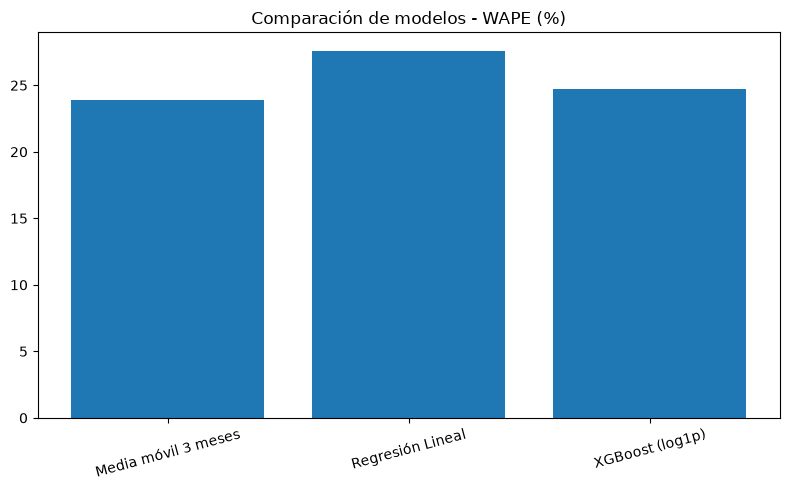
\includegraphics[width=0.75\textwidth]{templatefigures/comparacion_WAPE_porcentaje}
    \caption{Comparación de WAPE entre los tres modelos candidatos (holdout final).}
    \label{fig:comparacion_wape}
\end{figure}

\subsubsection{Consistencia mediante validación cruzada temporal}

Despues de obtener los resultados anteriores, se propuso el uso de una validacion cruzada para descartar que el resultado obtenido dependiera de las condiciones y particularidades de un unico periodo de prueba.

La idea principal, es probar el modelo varias veces simulando estar en un mes distinto al pasado, para poder evaluar si acierta de forma consistente y no solo una vez por casualidad. Para poder predecir un mes, solo se puede usar los meses que vinieron antes, no se pueden usar los datos que serian "Futuros", porque queremos simular un escenario real, y en ese caso, no se tendria esa informacion.


\begin{enumerate}
    \item Prueba 1 (Fold 1): Es el mas antiguo, se le enseña al modelo con los primeros 4 meses del año (Enero, febrero, Marzo, Abril), y se hace que el sistema adivine Mayo, Junio y Julio. Se compara lo que adivino contra los resultados reales de esos meses y se registra que tan grande fue el error.
    \item Prueba 2 (Fold 2): En este segunda prueba o Fold, se le enseña al modelo con 5 meses en ves de 4, es decir, de enero a Mayo, y se le pide que prediga Junio, Julio y agosto, una vez mas, se comparar y se registra el error.
    \item Prueba 3 (Fold 3): Por ultimo, se le enseña al modelo con 6 meses de Enero a junio y se le solicita al sistema que prediga julio , agosto y septiembre, se compara y, una vez mas, se registra el error.
\end{enumerate}


Dicha validacion cruzada temporal se implemento en el sistema en el archivo \texttt{app/services/prediccion/validacion.py}.

\begin{minted}{python}
TEST_SIZE_MESES = 3
MIN_TRAIN_MESES = 3
MAX_FOLDS = 3


def _armar_folds(meses_ordenados):
    n = len(meses_ordenados)
    folds = []
    fin_test = n
    while len(folds) < MAX_FOLDS:
        inicio_test = fin_test - TEST_SIZE_MESES
        if inicio_test < MIN_TRAIN_MESES:
            break
        folds.append((meses_ordenados[:inicio_test], meses_ordenados[inicio_test:fin_test]))
        fin_test -= 1
    folds.reverse()
    return folds
\end{minted}

Se definen tres constantes, \texttt{TEST\_SIZE\_MESES}, \texttt{MIN\_TRAIN\_MESES} y \texttt{MAX\_FOLDS}, que definen el tamaño de la ventana de prueba, el tamaño minimo de la ventana de entrenamiento y el numero maximo de folds a generar, respectivamente.


Se arma la funcion que genera las particiones \texttt{\_armar\_folds}, esta recibe una lista de todos los meses disponibles organizados cronologicamente. Se define el fold mas reciente, es decir, los ultimos meses disponibles \texttt{TEST\_SIZE\_MESES}. En cada iteracion se retrocede el punto de corte de un mes hacia atras en el tiempo, de esta manera, se crea un nuevo Fold cuyo entrenamiento crece en un mes respecto al anterior. Este proceso se repite hasta completar \texttt{MAX\_FOLDS}, o hasta que ya no quede suficiente historial y el tamaño de la ventana de entrenamiento sea menor a \texttt{MIN\_TRAIN\_MESES} meses de entrenamiento.  

Al finalizar, los folds se ordenan en orden cronologico del mas antiguo al mas nuevo antes de ser devueltos.

Al ya tener los folds organizados, el sistema entrena nuevamente los tres modelos candidatos, y selecciona el mejor modelo por producto, evaluando el resultado bajo la etiqueta de "Sistema final". Es decir, es la estrategia que usa Thary para predecir el consumo, en ves de escoger uno solo, para cada producto, el sistema entrena los 3 modelos y selecciona el que se equivoco menos conese producto en particular. El proceso se repite producto por producto.

Un aspecto importante es que, la eleccion de que modelo usar para cada producto se hace solo con los datos de entrenamiento, antes de ver los datos de prueba. Esto demuestra que no se esta "haciendo trampa, ya que el sistema no tiene acceso a los datos de prueba, y por lo tanto, no puede "aprender" de ellos.

Aun asi, solo esto no basta para confiar en el resultado, ya que aun si el sistema esta eligiendo el modelo de forma honesto, un unico experimento podria haber salido bien por casualidad y no porque el sitema de verdad sea bueno.


Es por eso que la validacion cruzada la aporto valor al sistema, ya que al repetir este mismo proceso (entrenamiento, eleccion del modelo y evaluacion) en diferentes periodos de prueba, se confirma que el resultado obtenido en el holdout final no fue un resultado aislado, sino que se repite de forma consistente en distintos periodos de prueba.

En la siguiente tabla se describen el promedio y la desviiacion estandar de las metricas obtenidas en cada fold, para cada modelo candidato y el sistema final:


\begin{table}[H]
    \centering
    \caption{Resumen de la validación cruzada temporal (promedio $\pm$ desviación, 3 folds).}
    \label{tab:resumen_cv}
    \begin{tabularx}{\textwidth}{Xcccc}
        \toprule
        \textbf{Modelo} & \textbf{MAE} & \textbf{RMSE} & \textbf{MAPE (\%)} & \textbf{WAPE (\%)} \\
        \midrule
        Media Móvil        & 44.27 $\pm$ 3.70  & 200.82 $\pm$ 41.31 & 82.38 $\pm$ 1.85  & 22.31 $\pm$ 1.29 \\
        Regresión Lineal   & 58.13 $\pm$ 2.21  & 270.35 $\pm$ 6.32  & 106.24 $\pm$ 10.64 & 29.38 $\pm$ 1.84 \\
        XGBoost            & 46.58 $\pm$ 3.46  & 223.64 $\pm$ 31.40 & 64.93 $\pm$ 2.25  & 23.48 $\pm$ 1.15 \\
        \textbf{Sistema final} & \textbf{36.25 $\pm$ 2.54} & \textbf{174.24 $\pm$ 27.89} & \textbf{59.13 $\pm$ 1.84} & \textbf{18.27 $\pm$ 0.81} \\
        \bottomrule
    \end{tabularx}
\end{table}

De la tabla se puede observar que:

De la tabla se puede observar que:

\begin{itemize}
    \item El sistema final es el que obtiene el mejor promedio en las cuatro metricas evaluadas, y tambien la menor desviacion estandar en todas ellas. Esto es significativo, porque demuestra que vale la pena la complejidad de elegir un modelo distinto para cada producto: el sistema final no solo es mas preciso en promedio, sino tambien mas consistente y estable entre los distintos periodos evaluados.
    \item La media movil es el segundo mejor modelo, seguido por XGBoost y finalmente la regresion lineal. Cuando se comparan los tres modelos candidatos de forma individual, la media movil es la que obtiene un mejor MAE, RMSE y WAPE, mientras que solo XGBoost la supera en MAPE. El hecho de que ninguno de los dos modelos mas sofisticados domine de forma general sobre la linea base avala la decision de seleccionar un modelo distinto por producto, ya que no existe un unico modelo que sea el mejor en todos los casos.
    \item La Regresion Lineal es la que tiene los peores resultados en las cuatro metricas, ademas de que su MAPE es el que mas varia entre los 3 folds. Esto es coherente con la tendencia de este modelo a sobreestimar los productos de alta demanda, observada previamente en el analisis de dispersion entre modelos, lo que ayuda a explicar por que su error resulta mas alto que el de los otros dos modelos.
    \item Finalmente, se observa que la efectividad del sistema final no se debe solamente a "elegir el mejor modelo en general", que en este caso seria la media movil, sino a elegir un modelo distinto para cada producto. En caso de haber elegido media movil para todos los productos, el error hubiera sido de 22.31\% de WAPE, mientras que al elegir el mejor modelo por producto, el error se reduce a 18.27\%.
\end{itemize}


\subsection{Evaluación de la Seguridad y Estándares}
% Guia: resultados del analisis de seguridad y nivel de cumplimiento de los
% estandares declarados en el capitulo 2.


\subsection{Análisis de Impactos de la Solución}
% Guia: impactos tecnicos, sociales, economicos, ambientales y eticos.


\subsection{Conclusiones}
% Guia: respuesta directa a los objetivos y a la pregunta de investigacion.


\subsection{Recomendaciones de Operación y Mantenibilidad}
% Guia: recomendaciones para la operacion, soporte y mantenibilidad del sistema.


\subsection{Trabajos Futuros}
% Guia: lineas de trabajo que quedan abiertas.


\subsection{Declaración de Uso Responsable de IA}
% Guia: declare que herramientas de IA se usaron, para que, y como se verifico
% el resultado.



%%%%%%%%%%%%%%%%%%%%%%%%%%%%%%%%%%%%%%%%%%%%%%%%%%%%%%%%%%%%%%%%%%%%%%%%%%%%%%%%%%%%%
%  REFERENCIAS  (estilo IEEE)
%  Se generan a partir de bibs/sample.bib; solo aparecen las que se citen
%  en el texto con \cite{...}.  Configuracion: template/bibliografia.tex
%%%%%%%%%%%%%%%%%%%%%%%%%%%%%%%%%%%%%%%%%%%%%%%%%%%%%%%%%%%%%%%%%%%%%%%%%%%%%%%%%%%%%

\cleardoublepage{}

% titlesec altera el funcionamiento interno de las secciones: sin este
% \phantomsection el enlace del indice apuntaria a la pagina equivocada
\phantomsection
\printbibliography[heading=bibintoc, title={Referencias Bibliográficas}]


%%%%%%%%%%%%%%%%%%%%%%%%%%%%%%%%%%%%%%%%%%%%%%%%%%%%%%%%%%%%%%%%%%%%%%%%%%%%%%%%%%%%%
%  ANEXOS
%%%%%%%%%%%%%%%%%%%%%%%%%%%%%%%%%%%%%%%%%%%%%%%%%%%%%%%%%%%%%%%%%%%%%%%%%%%%%%%%%%%%%
\clearpage
% TODO: contenido de los anexos A-E



\end{document}


